\documentclass[1pt]{article}
\usepackage {tikz}
\usetikzlibrary {arrows,automata}
\usepackage{amssymb}
\usepackage{listings}
\usepackage{pdfpages}
\usepackage{caption}
\usepackage[nottoc]{tocbibind}
\usepackage[T1]{fontenc}

\usepackage{amsmath}

\def\X#1{$#1$ &\tt\string#1}
\newcommand\tab[1][1cm]{\hspace*{#1}}

\makeatletter
\let\@fnsymbol\@arabic
\makeatother
\title{\huge \textrm{Dijkstra and Negative Arches}}
\date{\textrm{Politecnico di Milano, \\17 October 2018}}


\begin{document}

	\pagenumbering{gobble}
	\begin{titlepage}
		\maketitle
	\end{titlepage}

	\pagenumbering{arabic}

	\newpage
	\section{Introduction to the Problem}
		We notice that Dijkstra's Algorithm can not be applied to graph with negative arches. We wonder whether we could solve the problem by adding to every arch the absolute value of the smallest arch, such that every arch has a weight $>= 0$.


	\section{Solution}
		The answer is no and it's easy to show why this solution doesn't work by showing a counter-example.\\ Consider the following graph:\\
		\begin{figure}[!htb]
		\center
			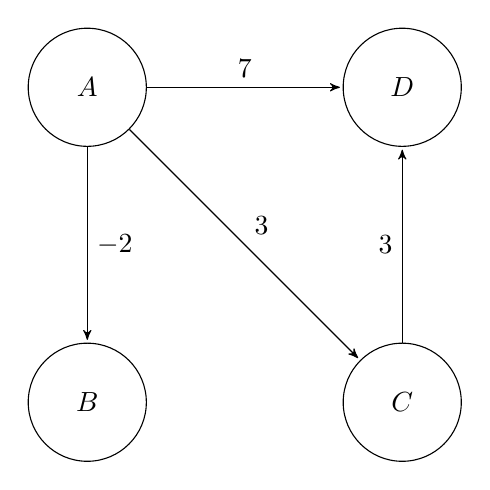
\begin{tikzpicture}[>=stealth',shorten >=1pt,auto,node distance=4cm, state/.style={circle, draw, minimum size=1.5cm}]
				\node[state] 		 (A)          {$A$};
				\node[state]         (D) [right of=A]   {$D$};
				\node[state]         (B) [below of=A]       {$B$};
				\node[state]         (C) [right of=B]      {$C$};


				\path[->] (A)   edge 			node {$7$}   (D)
								edge 			node {$3$}   (C)
								edge 			node {$-2$}   (B)
						  (C)	edge 			node {$3$}   (D);
						
			\end{tikzpicture}
		\end{figure}
		\\We want to find the shortest path between A and D. It is trivial to see that the shortest path is \emph{A-C-D} with a cost of $3+3=6$.\\
		If we apply the algorithm described in the above section, the graph would become:
				\begin{figure}[!htb]
		\center
			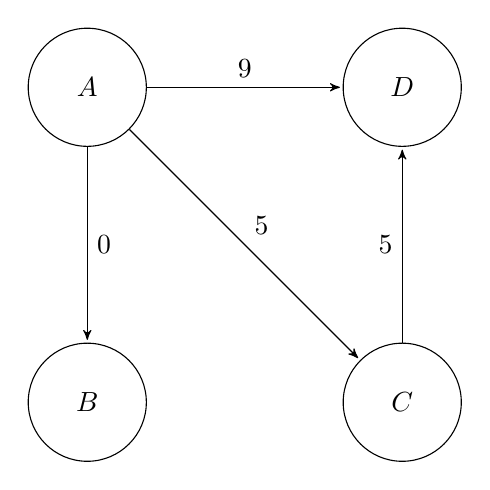
\begin{tikzpicture}[>=stealth',shorten >=1pt,auto,node distance=4cm, state/.style={circle, draw, minimum size=1.5cm}]
				\node[state] 		 (A)          {$A$};
				\node[state]         (D) [right of=A]   {$D$};
				\node[state]         (B) [below of=A]       {$B$};
				\node[state]         (C) [right of=B]      {$C$};


				\path[->] (A)   edge 			node {$9$}   (D)
								edge 			node {$5$}   (C)
								edge 			node {$0$}   (B)
						  (C)	edge 			node {$5$}   (D);
						
			\end{tikzpicture}
		\end{figure}
		\newpage
		We can easily see that the path \emph{A-C-D} now has a cost of $5+5=10$, therefore it's not the shortest path anymore. In this graph \emph{A-D} seems to be the shortest path.\\
		That occurs because we are adding the cost to the single arch and not to the path in its whole: adding the same value to the possible paths wouldn't change the shorter path since we are just "shifting" the solutions. A path is composed of several arches, that's why adding the same cost to each arch does not lead to the same solution.


\end{document}